\documentclass{beamer}

\title{PageRank}
\author{Ben Burns, Dan Magazu, Lucas Chagas, \\Thomas Webster, Trung Do}
\date{Fall 2021}

\usepackage{outlines}
\usepackage{graphicx}
\graphicspath{{./images}}

\addtobeamertemplate{navigation symbols}{}{%
    \usebeamerfont{footline}%
    \usebeamercolor[fg]{footline}%
    \hspace{1em}%
    \insertframenumber/\inserttotalframenumber
}

\begin{document}

\frame{\titlepage}

\begin{frame}
\frametitle{Table of Contents}
\tableofcontents
\end{frame}

\section{Motivation}
\begin{frame}[t]
\frametitle{Motivation}
\begin{itemize}
    \setlength\itemsep{0.5em}
    \item Problem: the internet has a \emph{lot} of web pages
    \item A lot of the information out there either isn't relevant to us, or is inaccurate
    \item Motivation: we want a program that, when provided a phrase, returns webpages with information relevant to the input
    \item Intuitive solution: return back websites that either contain that phrase, or contain similar phrases
    \item This helps us find more \emph{relevant} pages, but we can't know if we're getting the best information (much less \emph{accurate} information) without manually going through each result
    \item We desire a stronger solution
\end{itemize}
\end{frame}

\section{Background}
\begin{frame}[t]
\frametitle{PageRank}
\begin{outline}
    \1 Invented by Sergey Brin and Larry Page (1998)\footnotemark 
        \2 Publication marks them becoming co-founders of Google  
    \1 Idea: we want some way to numerically score each webpage based on how "important" it is
    \1 Algorithm numerically scores each page $p$ based on 
        \2 How many other pages link to $p$ (or "cite" it)
        \2 The "importance" of each of $p$'s citations 
    \1 We then numerically order pages to rank them
    \1 PageRank: the procedure for scoring each website
    \1 Google: the database that indexes the PageRank of each website for search
\end{outline}
\footnotetext[1]{Many use the year of the original manuscript, 1996}
\end{frame}

\begin{frame}[t]
\frametitle{Underlying Assumption}    
\begin{outline}
    \1 Running our basic search engine gives us a collection of pages with information relevant to our query
    \1 Assumption: More "important" and useful websites will be the ones with proportionally more inbound links
    \1 Pages with very reliable, primary information are likely to be cited by lots of website authors, and therefore will have lots of "flow" into them
%    \1 If what you're looking for is very niche and therefore won't have many inbound links, the best results will still have proprotionally more citations than other relevant sources
\end{outline}
\end{frame}

\begin{frame}[t]
\frametitle{Finding Less Important Information}
\begin{outline}
    \1 A worry you may have is that we'll only find pages with lots of inbound links
    \1 You can still find niche information by making your query more specific so that it won't match more general pages
    \1 Searching "PageRank" will likely get you Wikipedia, but "Anatomy of PageRank architecture" gives you the original research literature. 
    \1 Your returned urls are still proportionally important results, your query just filtered out the numerically more "important", yet less relevant pages.
\end{outline}
\end{frame}

\section{Formalizing PageRank}
\begin{frame}[t]
\frametitle{Formalizing the PageRank problem}
\begin{outline}
    \1 We're going to construct a directed graph $G = (V, E)$
    \1 For each website we consider, we construct a node $v_i \in V$
    \1 For two distinct nodes $v_i,\ v_j \in V$, the \emph{directed} edge $v_iv_j \in E$ iff there is a link on website $i$ that goes to website $j$.
    \1 If $v_i$ and $v_j$ are not distinct (a website is linking to itself), we ignore the link and do not construct a loop edge.
        \2 $G$ is not a psuedograph
    \1 Multiple hyperlinks on page $i$ to page $j$ are all represented by the single, directed edge 
        \2 $G$ is not a multigraph.
\end{outline}
\end{frame}

\begin{frame}
\frametitle{Visual Representation}
\begin{center}
    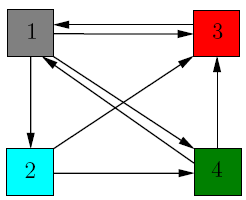
\includegraphics[width=0.6\textwidth]{unweighted.png}
\end{center}
\begin{outline}
    \1 We have a set of 4 websites
    \1 Each edge represents a hyperlink from the origin node to the destination node 
\end{outline}
\end{frame}

%\frametitle{Adjacency Matrix}
%\begin{columns}
    %\begin{frame}
%    \begin{column}{0.5\textwidth}
%        \centering
%        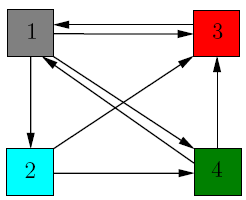
\includegraphics[width=\textwidth]{unweighted.png}
%    \end{column}
%    \begin{column}{0.5\textwidth}
%        \centering
%        {\Large$A = \begin{pmatrix}
%            0 & 1 & 1 & 1\\
%            0 & 0 & 1 & 1\\
%            1 & 0 & 0 & 0\\
%            1 & 0 & 1 & 0\\
%        \end{pmatrix}$}
%    \end{column}
%\end{columns}
%\begin{outline}
%    \1 No self loops means the main diagonal is all zeros
%\end{outline}
%\end{frame}

\begin{frame}[t]
\frametitle{Applying PageRank Values}
\begin{outline}
    \1 At first, we assign each vertex $v\in V$ with a weight of $\dfrac{1}{|V|}$. 
    \1 All vertices have equal weight, and our weights sum up to 1. The weight of a particular vertex $v_i$ is denoted $PR(v_i)$.
    \1 Consider the set $V_i$ of vertices that $v_i$ has an edge to:
        \2 $V_i = \{v_j | v_iv_j \in E\}$
    \1 A user on page 1 can choose to click a link to traverse to either 2, 3, or 4. In other words, $V_1 = \{2, 3, 4\}$.
%    \1 For each vertex in the set, the weight of the edge to that vertex will be the PageRank value of the source node divided by the number of outbound edges it has
%        \2 $\forall v_j \in V_i: w(v_iv_j) = \dfrac{PR(v_i)}{|V_i|}$
%    \1 In other words, all the outbound edges from a particular vertex will have the same weight
\end{outline}
\begin{center}
    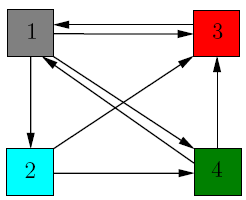
\includegraphics[width=0.4\textwidth]{unweighted.png}
\end{center}
\end{frame}

\begin{frame}[t]
\frametitle{Traversing from Page to Page}
\begin{itemize}
    \setlength\itemsep{1em}
    \item Assumption: A user on page $i$ user is equally likely to choose to visit each vertex in $V_i$ (our set of vertices that $v_i$ cites)
    \item From $v_i$, $P(v_j) = \dfrac{1}{|V_i|}$ if $v_j \in V_i$, and 0 else.
    \item In our example from before, the probabilty that our user on page 1 visits page 2 is $P(v_2) = \dfrac{1}{|V_1|} = \dfrac{1}{3}$
    \item So a third of page 1's visitors will "flow" to page 2, a third to page 3, and a third to page 4
\end{itemize}
\end{frame}

\begin{frame}[t]
\frametitle{Iteration Model}
\begin{outline}
    \1 All at once, all users will click one of the links on their curreny page
    \1 At click 0, the PageRank value of all vertices $PR(v) = \dfrac{1}{|V|}$
    \1 On click 1, each page will equally split its PageRank value among the pages it cites
    \1 Page 1 starts with $PR(v_1) = \dfrac{1}{4}$ at click 0, and contributes $\dfrac{1}{12}$ to each of 2, 3, and 4 on click 1
    \1 Conversely, page 1 will receive nothing from page 2, all of $PR(v_3)$, and half of $PR(v_4)$. So after click 1, $PR(v_1) = 0\cdot PR(v_2) + PR(v_3) + \dfrac{1}{2}PR(v_4) = \dfrac{1}{4} + \dfrac{1}{8} = \dfrac{3}{8}$
    \1 After click $n$, $PR(v_1) = \dfrac{1}{|V_2|}PR(v_2) + \dfrac{1}{|V_3|}PR(v_3) + \dfrac{1}{|V_4|}PR(v_4)$
\end{outline}
\end{frame}


%\begin{frame}
%\frametitle{Visual Representation}
%\begin{center}
%    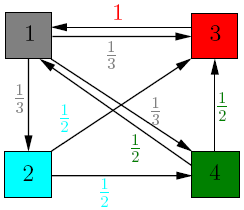
\includegraphics[width=0.6\textwidth]{weighted.png}
%\end{center}
%\begin{outline}
%    \1 In this case, all nodes have a PageRank value of 1.
%\end{outline}
%\end{frame}

%\begin{frame}
%\frametitle{Transition Matrix}
%\begin{columns}
%    \begin{column}{0.5\textwidth}
%        \centering
%        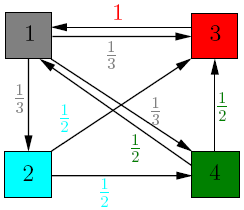
\includegraphics[width=\textwidth]{weighted.png}
%    \end{column}
%    \begin{column}{0.5\textwidth}
%        \centering
%        $T = \begin{pmatrix}
%            0 & 1/3 & 1/3 & 1/3\\
%            0 & 0 & 1/2 & 1/2\\
%            1 & 0 & 0 & 0\\
%            1/2 & 0 & 1/2 & 0\\
%        \end{pmatrix}$
%    \end{column}
%\end{columns}
%\begin{outline}
%    \1 All entries of the transition matrix are non-negative
%    \1 If $v_i$ has at least one outgoing edge, the sum of the entries in row $i$ is 1
%        \2 Else, the sum is 0.
%\end{outline}
%\end{frame}


\end{document}